\section{Application}

\subsection{Formulating the Shortest-Path Problem} \label{app:formulating}

One common problem in the context of computer science is the shortest-path-in-graph/network problem. Algorithms such as Dijkstra's algorithm exist and run much faster asymptotically than the Simplex Method, but they do not use linear algebra techniques like the Simplex Method does. Consider a weighted, directed graph $G = (V,E)$ (a set of vertices $V$ and edges $E$), where $w_{uv} \geq 0$ is the weight of the edge connecting from vertex $u$ to vertex $v$ or 0 if there is no edge connecting from $u$ to $v$.

Now consider the problem of finding the shortest path between two vertices in this graph. Finding the shortest path in the graph is solvable through the Simplex Method by formulating the problem as minimizing the cost of flow between two vertices $s$ and $t$\textsuperscript{[1]}:

\begin{equation}
    \begin{array}{rcl}
        \text{minimize}\ & & \sum_{(u,v) \in E} w_{uv} f_{uv} \\
        \text{subject to}\ \sum_{u \in V} f_{vu} - \sum_{w \in V} f_{wv} & = &
        \begin{cases} 
            1 & v = s \\
            -1 & v = t \\
            0 & \text{otherwise}
        \end{cases} \\
        \text{where}\ f_{uv} \geq 0 & \forall & (u,v) \in E
    \end{array}
\end{equation}

The reasoning behind the constraints is that we want conservation of flow along all vertices except for the source and target vertices. Hence, we want the outtake of a vertex minus the intake of a vertex to be 0. Likewise, we want the source to have an output flow of 1 and the target to have an input flow of 1 so that we find the minimum flow from the source vertex to the target vertex. The objective function then serves to minimize the weights of the edges along which this flow occurs.

A solution will have $f_{uv} = 1$ if edge $(u,v)$ is in the shortest path, and $f_{uv} = 0$ if not. To convert this into standard form (assuming $|V| = n$ vertices), we will write this system with variables $f_{uv}\ \forall\ u,v \in V$ so that $A \in \mathcal{M}_{n,n^2}, \mathbf{b} \in \mathbb{R}^n,$ and $\mathbf{c} \in \mathbb{R}^{n^2}$. To make generating the matrix $A$ and vectors $\mathbf{b}, \mathbf{c}$ simpler, we let the value of every vertex $v \in V$ be $0, 1, \cdots, n-1$. Then, for vertices $u,v \in V$, we let $i = v$ be the row of the constraint for vertex $v$ and $j = un + v$ be the column for variable $f_{uv}$ for $A_{ij}$. (This also makes extracting solutions for edges $(u,v)$ from indices of $\mathbf{c}$ easy since for $c_j$, vertex $u = \lfloor j / n \rfloor$ and vertex $v = j\ \text{mod}\ n$.)

Since we wish to minimize the shortest path, we will have to solve the dual simplex problem for this system; that is (using $A, \mathbf{b},$ and $\mathbf{c}$ above),

\begin{equation} %\label{eq:linprog}
    \begin{array}{rrcl}
        \text{maximize} & \mathbf{b}^\text{T} \mathbf{y} \\
        \text{subject\ to} & A^\text{T} \mathbf{y} & \leq & \mathbf{c} \\
        \text{where} & \mathbf{y} & \geq & \mathbf{0}
    \end{array}
\end{equation}

and the solution $\mathbf{x}$ obtained from the dual simplex method will be the solution to the minimum problem. Then, $\forall\ j: x_j = 1$, edge $(u,v)$ (once again, where $u = \lfloor j / n \rfloor$ and $v = j\ \text{mod}\ n$) will be in the shortest path.

\subsection{Simple Example}

Consider the following graph, with the edge weights denoted along their respective edges:

\begin{center}
    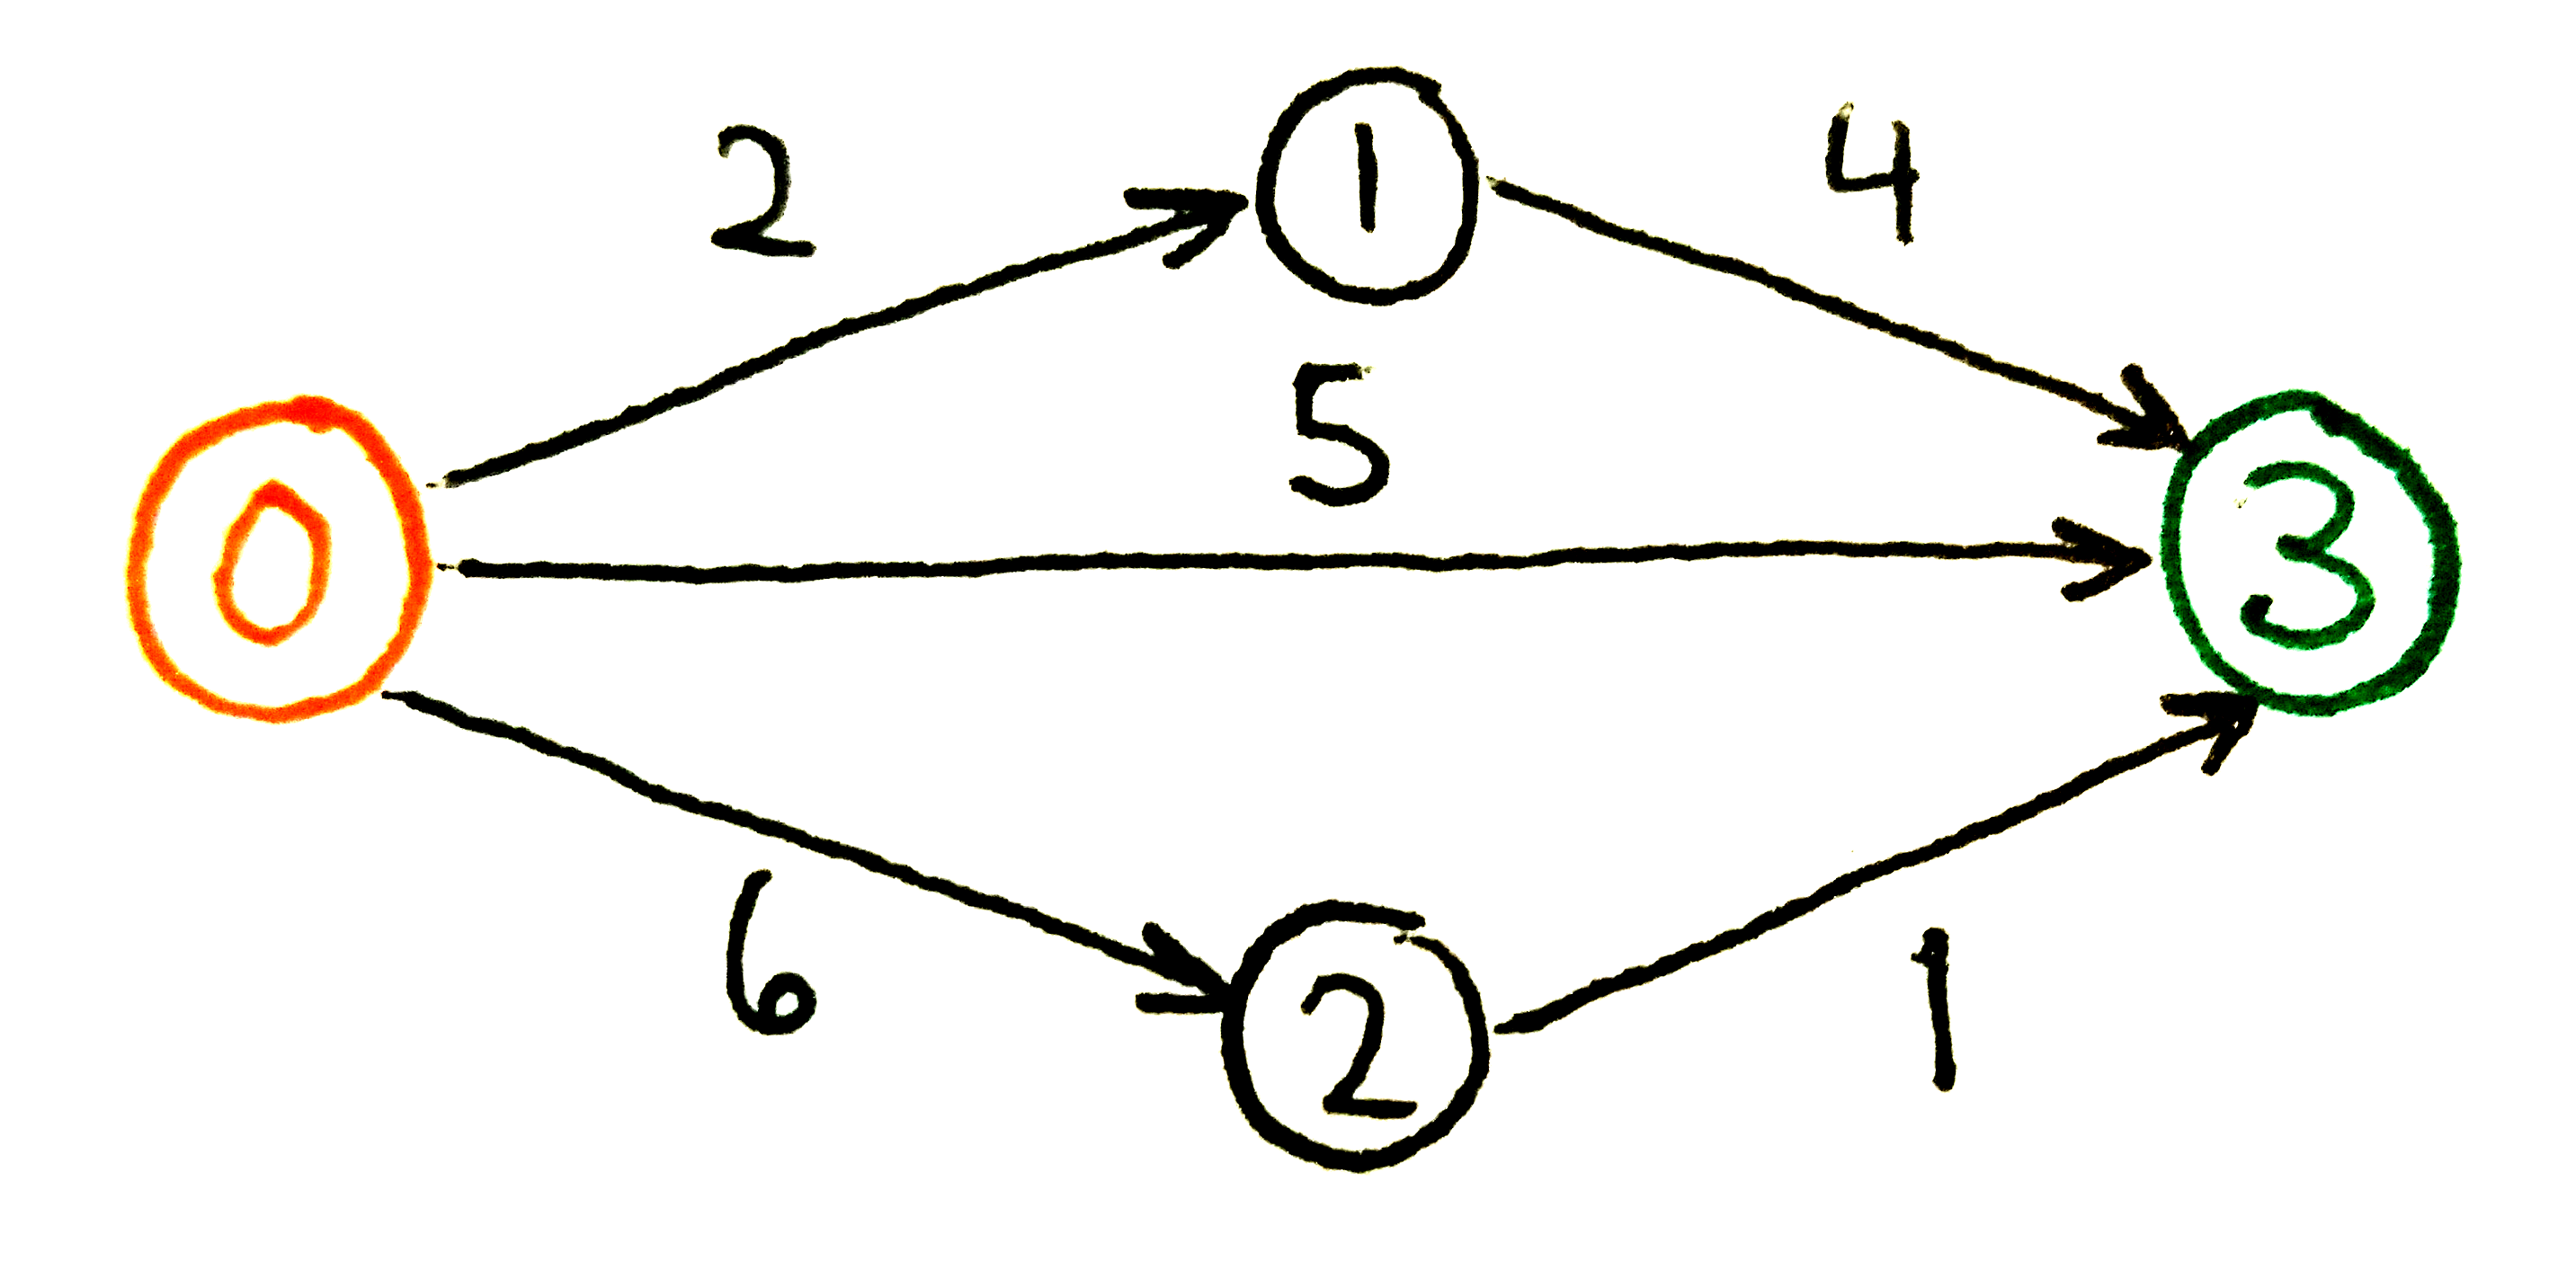
\includegraphics[width=2.33in]{simple}
\end{center}

We want to find the shortest path from vertex 0 to vertex 3. Clearly, the shortest path is directly from vertex 0 to vertex 3, but we will use this observation to verify the validity of the formulation from section \ref{app:formulating}. Using that formulation:

\begin{equation*}
    A = 
    \begin{pmatrix}
        0 & 1 & 1 & 1 & 0 & 0 & 0 & 0 & 0 & 0 & 0 & 0 & 0 & 0 & 0 & 0\\
        0 & -1 & 0 & 0 & 0 & 0 & 0 & 1 & 0 & 0 & 0 & 0 & 0 & 0 & 0 & 0\\
        0 & 0 & -1 & 0 & 0 & 0 & 0 & 0 & 0 & 0 & 0 & 1 & 0 & 0 & 0 & 0\\
        0 & 0 & 0 & -1 & 0 & 0 & 0 & -1 & 0 & 0 & 0 & -1 & 0 & 0 & 0 & 0
    \end{pmatrix}
\end{equation*}
\begin{equation*}
    \mathbf{b} = 
    \begin{pmatrix}
        1 & 0 & 0 & -1
    \end{pmatrix}^\text{T}
\end{equation*}
\begin{equation*}
    \mathbf{c} = 
    \begin{pmatrix}
        0 & 2 & 6 & 5 & 0 & 0 & 0 & 4 & 0 & 0 & 0 & 1 & 0 & 0 & 0 & 0
    \end{pmatrix}^\text{T}
\end{equation*}

Using the dual simplex method we implemented (see Appendix \ref{appendix:code} for the implementation) to find the minimum path, we get the solution:
\begin{equation*}
    \mathbf{x} = 
    \begin{pmatrix}
        0 & 0 & 0 & 1 & 0 & 0 & 0 & 0 & 0 & 0 & 0 & 0 & 0 & 0 & 0 & 0
    \end{pmatrix}^\text{T}
\end{equation*}

This indicates that there is only one edge along the shortest path. Using the fact that, for index $j$ in $c_j$, the corresponding edge $(u,v)$ is $u = \lfloor j / n \rfloor$ and $v = j\ \text{mod}\ n$, we see that the only edge along the shortest path is $(\lfloor 3 / 4 \rfloor, 3\ \text{mod}\ 4) = (0,3)$ (since indexing starts at 0 in Python). This is what we expected from our earlier observation.

\subsection{Finding Shortest Route from Fleming to Duane}

Finding a quick path from one building to another on the campus of CU Boulder can be difficult with how much sidewalk there is, and the campus is so large that finding one is essential to making it to class on time. Many engineering students find themselves rushing from Fleming Law to Duane Physics and vice versa on a daily basis, so finding the shortest path between the two buildings would be ideal.

Since we are good students, we would never walk on the grass and ruin the landscape or vault over fences and such; we will only walk on the sidewalks in between classes. The following graph is a good approximation of the sidewalk between Fleming Law and Duane Physics (where Fleming is at vertex 0 and Duane is at vertex 49):

\begin{center}
    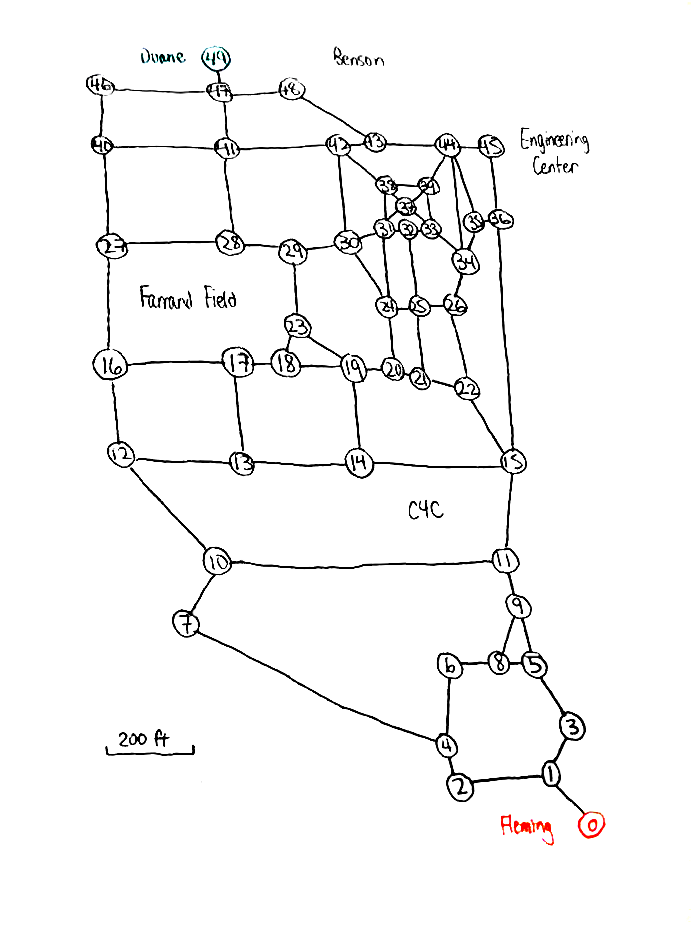
\includegraphics[width=3.5in]{map}
\end{center}

The edge weights, in this case, are the distances between vertices. This graph is also undirected, meaning that for $(u,v) \in E$, $w_{uv} = w_{vu}$ (and therefore we can convert it to a directed graph by adding an edge from $u$ to $v$ and from $v$ to $u$).

Since $|V| = 50$ vertices, $A \in \mathcal{M}_{50,2500}$, $\mathbf{b} \in \mathbb{R}^{50}$, and $\mathbf{c} \in \mathbb{R}^{2500}$, which is too much information to display on this page. We created the graph in \texttt{campusgraph.py} using NetworkX, a graph library for Python, and used the graph created in this Python file to generate $A$, $\mathbf{b}$, and $\mathbf{c}$ (see \texttt{shortestpath.py} for implementation) to solve the problem, using the formulation in section \ref{app:formulating} and the dual simplex method. We let the source be vertex 0 (Fleming) and the target be vertex 49 (Duane), but the shortest path will be the same in either direction since the graph is undirected.

\texttt{shortestpath.py} extracted the edges from the solution vector $\mathbf{x}$ and outputted the following shortest path as an edge list:

\small{\texttt{(0, 1), (1, 3), (3, 5), (5, 9), (9, 11), (11, 15), (15, 22), (22, 26), (26, 34), (33, 37), (34, 33), (37, 38), (38, 42), (41, 47), (42, 41), (47, 49)}}

This corresponds to the following path:

\begin{center}
    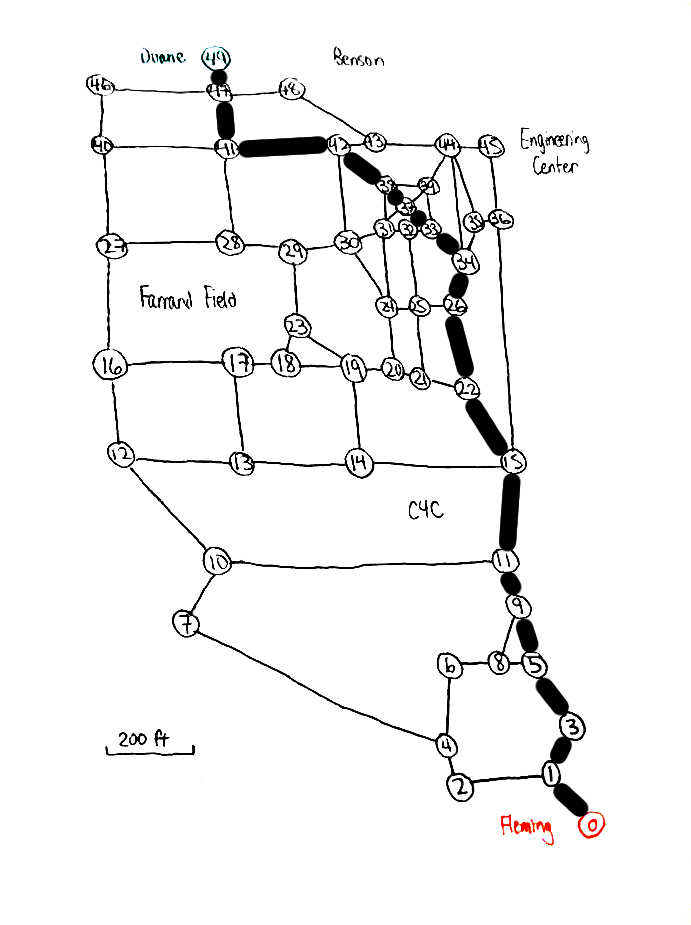
\includegraphics[width=3.5in]{map_sp}
\end{center}

Therefore, we can conclude that the shortest path from Fleming to Duane (walking on sidewalks only) is as follows: from Fleming, walk directly to the Regent Underpass and continue straight along the sidewalk until reaching Crosman Hall. Then go between Crosman and Reed and continue on the diagonal sidewalk. Once the end of the diagonal sidewalk is reached, walk toward JILA until there is sidewalk on the right, which leads to Duane.

\begin{thebibliography}{9}

\bibitem{chandrasekaran}
Chandrasekaran, R. 
\textit{Shortest Path.} 
\url{https://www.utdallas.edu/~chandra/documents/networks/net3.pdf}

\bibitem{ferguson}
Ferguson, T. S.
\textit{Linear Programming.}
\url{https://www.math.ucla.edu/~tom/LP.pdf}

\bibitem{gale}
Gale, D.
\textit{Linear Programming and the Simplex Method.}
Notices of the AMS. 
Volume 54, Number 3.
\url{https://www.ams.org/notices/200703/fea-gale.pdf}

\bibitem{trevisan}
Trevisan, L.
\textit{Lecture 6 Notes.}
\url{https://people.eecs.berkeley.edu/~luca/cs261/lecture06.pdf}

\end{thebibliography}

\newpage
\appendix
\section{Python Code} \label{appendix:code}

Note: we used the \texttt{numpy} package for its linear algebra functionality, and we used the \texttt{networkx} package to create the graphs.

\underline{\texttt{main.py}}
\begin{verbatim}
import campusgraph
import networkx as nx
from shortestpath import *

def simple_example():
    G = nx.DiGraph()
    G.add_edge(0, 1, weight=2.)
    G.add_edge(0, 2, weight=6.)
    G.add_edge(0, 3, weight=5.)
    G.add_edge(1, 3, weight=4.)
    G.add_edge(2, 3, weight=1.)
    p = shortest_path(G, 0, 3)
    print(p)

def campus_problem():
    G = campusgraph.create_graph()
    p = shortest_path(G, 0, 49)
    print(p)

def main():
    simple_example()
    print()
    campus_problem()

if __name__ == '__main__':
    main()
\end{verbatim}

\newpage
\underline{\texttt{simplex.py}}
\begin{scriptsize}
\begin{verbatim}
# -*- coding: utf-8 -*-
"""
Simplex Algorithm

"""

import numpy as np

class Tableau:    
    def __init__(self, mrows, ncols):
        self.m = mrows
        self.n = ncols
        self.b = np.zeros((1, mrows))
        # 1x a placeholder for left col, y's
        self.t = np.arange(10, 10+mrows, 1)
        # 2x a placceholder for top row, x's
        self.r = np.arange(20, 20+ncols, 1)
        self.c = np.zeros((1, ncols))
        self.a = np.zeros((mrows, ncols))
        self.objVal = 0
    
    def pivot(self, i, j):
        if self.a[i,j] == 0:
            raise Exception("Pivot error: a[i,j] must not be 0")
        tmp = self.r[j]
        self.r[j] = self.t[i]
        self.t[i] = tmp
        #calculate new coefficients for matrix
        ahat = np.copy(self.a)
        for n in range(0,self.m):
            for k in range(0,self.n):
                if n==i and k==j:
                    ahat[n,k] = 1/self.a[i,j]
                elif n==i:
                    ahat[n,k] /= self.a[i,j]
                    
                elif k==j:
                    ahat[n,k] /= -self.a[i,j]
                else:
                    ahat[n,k] -= self.a[i,k]*self.a[n,j]/self.a[i,j]
        # calculate new b values
        bhat = np.copy(self.b)
        for n in range(0, self.m):
            if n==i:
                bhat[n] /= self.a[i,j]   
            else:
                bhat[n] -= self.b[i]*self.a[n,j]/self.a[i,j]
        # calculate new cost values
        chat = np.copy(self.c)
        for k in range(0, self.n):
            if k==j:
                chat[k] /= -self.a[i,j]
            else:
                chat[k] -= self.a[i,k]*self.c[j]/self.a[i,j]
        # set new tableau
        self.objVal -= self.b[i]*self.c[j]/self.a[i,j]
        self.a = ahat
        self.b = bhat
        self.c = chat
    
    def simplex(self):
    # Use simplex pivot rules until we either find the solution (-c_j >= 0)
    # or we find the problem is unbounded feasible (all a_ij<=0 for -c_j<0)
        while np.any(self.c < 0):
            # Case I: b >= 0
            if np.all(self.b >= 0):
                pivot_cols = np.where(self.c < 0)[0]
                
                # Create list of possible pivots and ratios b_i/a_ij
                poss_pivots = []
                poss_pivot_ratios = []
                for col in pivot_cols:
                    rows = np.where(self.a[:,col] > 0)[0]
                    for row in rows:
                        # Push tuple of row,col to pivots list
                        poss_pivots.append((row, col))
                        poss_pivot_ratios.append(self.b[row]/self.a[row,col])
                
                if len(poss_pivots) == 0:
                    raise Exception("Problem is unbounded feasible")
                min_ratio_index = np.argmin(poss_pivot_ratios)
                curr_pivot = poss_pivots[min_ratio_index]

                # Now pivot at the pivot we've chosen
                self.pivot(curr_pivot[0], curr_pivot[1])
            # Case II: some b_i < 0
            else:
                k = np.where(self.b < 0)[0][0] # b_k is first b_i<0
                neg_a_kj0 = np.where(np.array(self.a[k,:])[0] < 0)[0]
                if len(neg_a_kj0) == 0:
                    raise Exception("Problem is infeasible")
                pivot_col = neg_a_kj0[0] # j_0 is the pivot column
                
                pivot_rows_1 = np.where(self.b >= 0)[0]
                pivot_rows_2 = np.where(np.array(self.a[:,pivot_col])[0] > 0)[0]
                # We want rows where both conditions are true, so get their intersection
                pivot_rows = np.append(np.intersect1d(pivot_rows_1, pivot_rows_2), [k])

                pivot_row_ratios = np.divide(self.b[pivot_rows],
                                                    self.a[pivot_rows,pivot_col].T)
                
                min_ratio_index = np.argmin(pivot_row_ratios)
                pivot_row = pivot_rows[min_ratio_index]

                # Now pivot at the pivot we've chosen
                self.pivot(pivot_row, pivot_col)
        
    # solution to maximum problem
    def getX(self):
        x = np.zeros((1, self.n))
        for k in range(0,self.n):
            if self.r[k] == 0:
                x[k] = 0
            else:
                for n in range(0, self.m):
                    if self.t[n] == 20+k:
                        x[0][k] = self.b[n]
        return(x[0])
    
    # solution to minimum problem
    def getY(self):
        y = np.zeros((1,self.m))
        for n in range(0, self.m):
            if self.t[n] == 0:
                y[n] = 0
            else:
                for k in range(0, self.n):
                    if self.r[k] == 10+n:
                       y[0][n] = self.c[k]
        return(y[0])
\end{verbatim}
\end{scriptsize}

\newpage
\underline{\texttt{shortestpath.py}}
\begin{verbatim}
import networkx as nx
import numpy as np
import simplex

def shortest_path(G, source, target):
# Find shortest path in graph G using the Simplex Method.
# Assume all nodes in G are labeled 0,1,2,...,n-1 where n is number of nodes
    # Create tableau for LP formulation
    n = len(G) # len(G) is number of nodes
    b = np.array(np.zeros((1, n)))[0]
    b[source] = 1; b[target] = -1
    A = np.zeros((n, n*n))
    c = np.array(np.zeros((1, n*n)))[0]
    for v in G.nodes():
        for u in G.predecessors(v):
            A[v][u*n + v] = -1
        for u in G.successors(v):
            A[v][v*n + u] = 1
            c[v*n + u] = G[v][u]['weight']

    # Now solve dual-simplex problem for shortest path
    t = simplex.Tableau(n*n,n)
    t.b = c
    t.a = A.T
    t.c = -b
    t.simplex()
    solution = t.getY()

    # Finally, extract path from solution
    path = []
    soln_indices = np.where(solution == 1)[0]
    for i in soln_indices:
        u = i // n
        v = i % n
        path.append((u,v))
    
    return path
\end{verbatim}

\newpage
\underline{\texttt{campusgraph.py}}
\begin{footnotesize}
\begin{verbatim}
import networkx as nx

def create_graph():
  # Node 0 is Fleming, Node 49 is Duane
  G = nx.DiGraph()
  G.add_edge(0, 1, weight=150.); G.add_edge(1, 2, weight=200.)
  G.add_edge(1, 3, weight=133.); G.add_edge(2, 4, weight=100.)
  G.add_edge(3, 5, weight=200.); G.add_edge(4, 6, weight=200.)
  G.add_edge(4, 7, weight=700.); G.add_edge(5, 8, weight=67.)
  G.add_edge(5, 9, weight=133.); G.add_edge(6, 8, weight=100.)
  G.add_edge(7, 10, weight=167.); G.add_edge(8, 9, weight=150.)
  G.add_edge(9, 11, weight=100.); G.add_edge(10, 11, weight=700.)
  G.add_edge(10, 12, weight=400.); G.add_edge(11, 15, weight=250.)
  G.add_edge(12, 13, weight=300.); G.add_edge(12, 16, weight=267.)
  G.add_edge(13, 14, weight=267.); G.add_edge(13, 17, weight=267.)
  G.add_edge(14, 15, weight=400.); G.add_edge(14, 19, weight=267.)
  G.add_edge(15, 22, weight=250.); G.add_edge(15, 36, weight=700.)
  G.add_edge(16, 17, weight=267.); G.add_edge(16, 27, weight=300.)
  G.add_edge(17, 18, weight=100.); G.add_edge(18, 19, weight=167.)
  G.add_edge(18, 23, weight=100.); G.add_edge(19, 20, weight=100.)
  G.add_edge(19, 23, weight=167.); G.add_edge(20, 21, weight=50.)
  G.add_edge(20, 24, weight=167.); G.add_edge(21, 22, weight=100.)
  G.add_edge(21, 25, weight=200.); G.add_edge(22, 26, weight=200.)
  G.add_edge(23, 29, weight=200.); G.add_edge(24, 25, weight=50.)
  G.add_edge(24, 30, weight=200.); G.add_edge(24, 31, weight=200.)
  G.add_edge(25, 26, weight=67.); G.add_edge(25, 32, weight=200.)
  G.add_edge(26, 34, weight=133.); G.add_edge(27, 28, weight=300.)
  G.add_edge(27, 40, weight=300.); G.add_edge(28, 29, weight=150.)
  G.add_edge(28, 41, weight=300.); G.add_edge(29, 30, weight=150.)
  G.add_edge(30, 31, weight=100.); G.add_edge(30, 42, weight=300.)
  G.add_edge(31, 32, weight=50.); G.add_edge(31, 37, weight=67.)
  G.add_edge(31, 38, weight=100.); G.add_edge(32, 33, weight=50.)
  G.add_edge(33, 34, weight=133.); G.add_edge(33, 37, weight=67.)
  G.add_edge(33, 39, weight=100.); G.add_edge(34, 35, weight=100.)
  G.add_edge(34, 44, weight=333.); G.add_edge(35, 36, weight=33.)
  G.add_edge(35, 44, weight=233.); G.add_edge(36, 45, weight=200.)
  G.add_edge(37, 38, weight=67.); G.add_edge(37, 39, weight=67.)
  G.add_edge(38, 39, weight=100.); G.add_edge(38, 42, weight=150.)
  G.add_edge(39, 44, weight=150.); G.add_edge(40, 46, weight=167.)
  G.add_edge(40, 41, weight=300.); G.add_edge(41, 42, weight=267.)
  G.add_edge(41, 47, weight=167.); G.add_edge(42, 43, weight=100.)
  G.add_edge(43, 44, weight=200.); G.add_edge(43, 48, weight=250.)
  G.add_edge(44, 45, weight=100.); G.add_edge(46, 47, weight=300.)
  G.add_edge(47, 48, weight=167.); G.add_edge(47, 49, weight=67.)
  # Shortest path algorithm for simplex method requires directed graph, but we
  # have undirected graph so we'll add backedge for every edge to make it
  # directed
  for e in G.edges():
    u,v = e
    G.add_edge(v, u, weight=G[u][v]['weight'])
  return G
\end{verbatim}
\end{footnotesize}

\end{document}